\documentclass[9pt, aspectratio=169]{beamer}
\usepackage{FiraSans}
\usetheme[subsectionpage=progressbar]{metropolis}
\usepackage[utf8]{inputenc}
\usepackage{amsmath}
\usepackage{amsfonts}
\usepackage{amssymb}
\usepackage{multicol}
\usepackage{tikz}
\usepackage{caption}
\usepackage{xcolor}
\usepackage[T1]{fontenc} 
\usepackage[skins]{tcolorbox}
\author{Nicola Roman\`o - nicola.romano@ed.ac.uk}
\title{Lecture 07 - Segmentation}
\setlength{\fboxsep}{0pt}
\setbeamertemplate {footline}{\begin{scriptsize}\hfill\insertframenumber ~of \inserttotalframenumber\kern1em\vskip5pt\end{scriptsize}}

% Remove "Figure" in front of captions
% See https://tex.stackexchange.com/questions/82456/how-to-remove-figure-caption-prefix-figure-in-beamer
\captionsetup{labelformat=empty,labelsep=none}

\titlegraphic{\centering 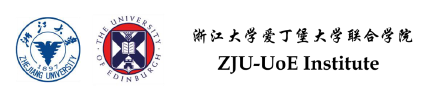
\includegraphics[scale=.5]{instituteLogo.png}}
\date{}

\begin{document}

\newtcolorbox{codebox}{enhanced,
    top=2pt,
    left=2pt,
    right=2pt,
    bottom=2pt,
    boxrule=0pt,
    leftrule=5pt,
    sharp corners,
    colback=gray!20,
    colframe=blue!60!black}

\begin{frame}
    \titlepage
\end{frame}

\begin{frame}
    {Learning objectives}
    \begin{columns}
        \begin{column}{0.8\textwidth}
            \begin{itemize}
                \item Describe the problem of segmentation
                \item Define and give examples of semantic and instance segmentation.
                \item Describe and use methods for semantic segmentation (thresholding, clustering, etc.)
                \item Describe and use methods for instance segmentation (watershed)
            \end{itemize}
        \end{column}
        \begin{column}{0.2\textwidth}
            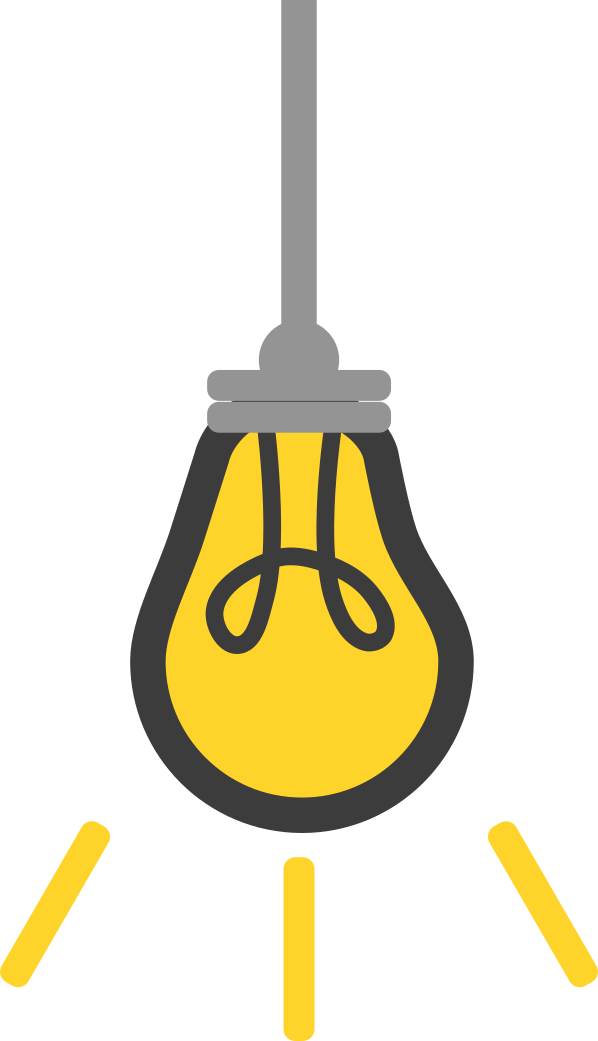
\includegraphics[angle=-30, origin=tr, width=1.5\textwidth]{lightbulb.png}
        \end{column}
    \end{columns}
\end{frame}

\section{Introduction}

\begin{frame}
    {Segmentation - definition}
    \begin{itemize}
        \item Segmentation is a long-studied (and complex!) problem in computer vision.
        \item Process of dividing an image into sets of pixels called \textit{segments} or \textit{objects}
        \item Each pixel gets a label identifying which object it belongs to.
        \item The different segments can then be analysed independently.
    \end{itemize}
\end{frame}

\begin{frame}
    {Application of segmentation}
    In biomedical imaging
    \begin{itemize}
        \item Segmentation of cells to measure their properties
        \item Analysis of X-ray images to identify pathologies
        \item Aid in surgery planning
    \end{itemize}
    \pause
    In computer vision in general
    \begin{itemize}
        \item Car, pedestrian, break lights detection (e.g. for autonomous car navigation)
        \item Face detection (e.g. for facial recognition, emotion analysis etc.)
        \item Fingerprint recognition
        \item \dots
    \end{itemize}
\end{frame}

\begin{frame}
    {Methods for segmentation}
    Segmentation is a difficult problem to solve, with many important practical applications, so it has been widely studied.

    \pause

    This lecture will cover some of the \textbf{traditional methods} for image segmentation. More recent \textbf{machine learning-based methods} will be covered later in the course.
\end{frame}

\begin{frame}
    {Semantic segmentation vs instance segmentation}
    There are two main types of segmentation:

    \begin{itemize}
        \item \textbf{Semantic segmentation}: divides the image in regions, each of which belongs to a specific class. Multiple objects of the same class will be detected in the same region.
        \item \textbf{Instance segmentation}: divides the image in regions, each of which is an instance of a class. Multiple objects of the same class will be detected as separate regions.
    \end{itemize}
\end{frame}

\begin{frame}
    {Semantic segmentation vs instance segmentation - an example}
    \only<1>{
        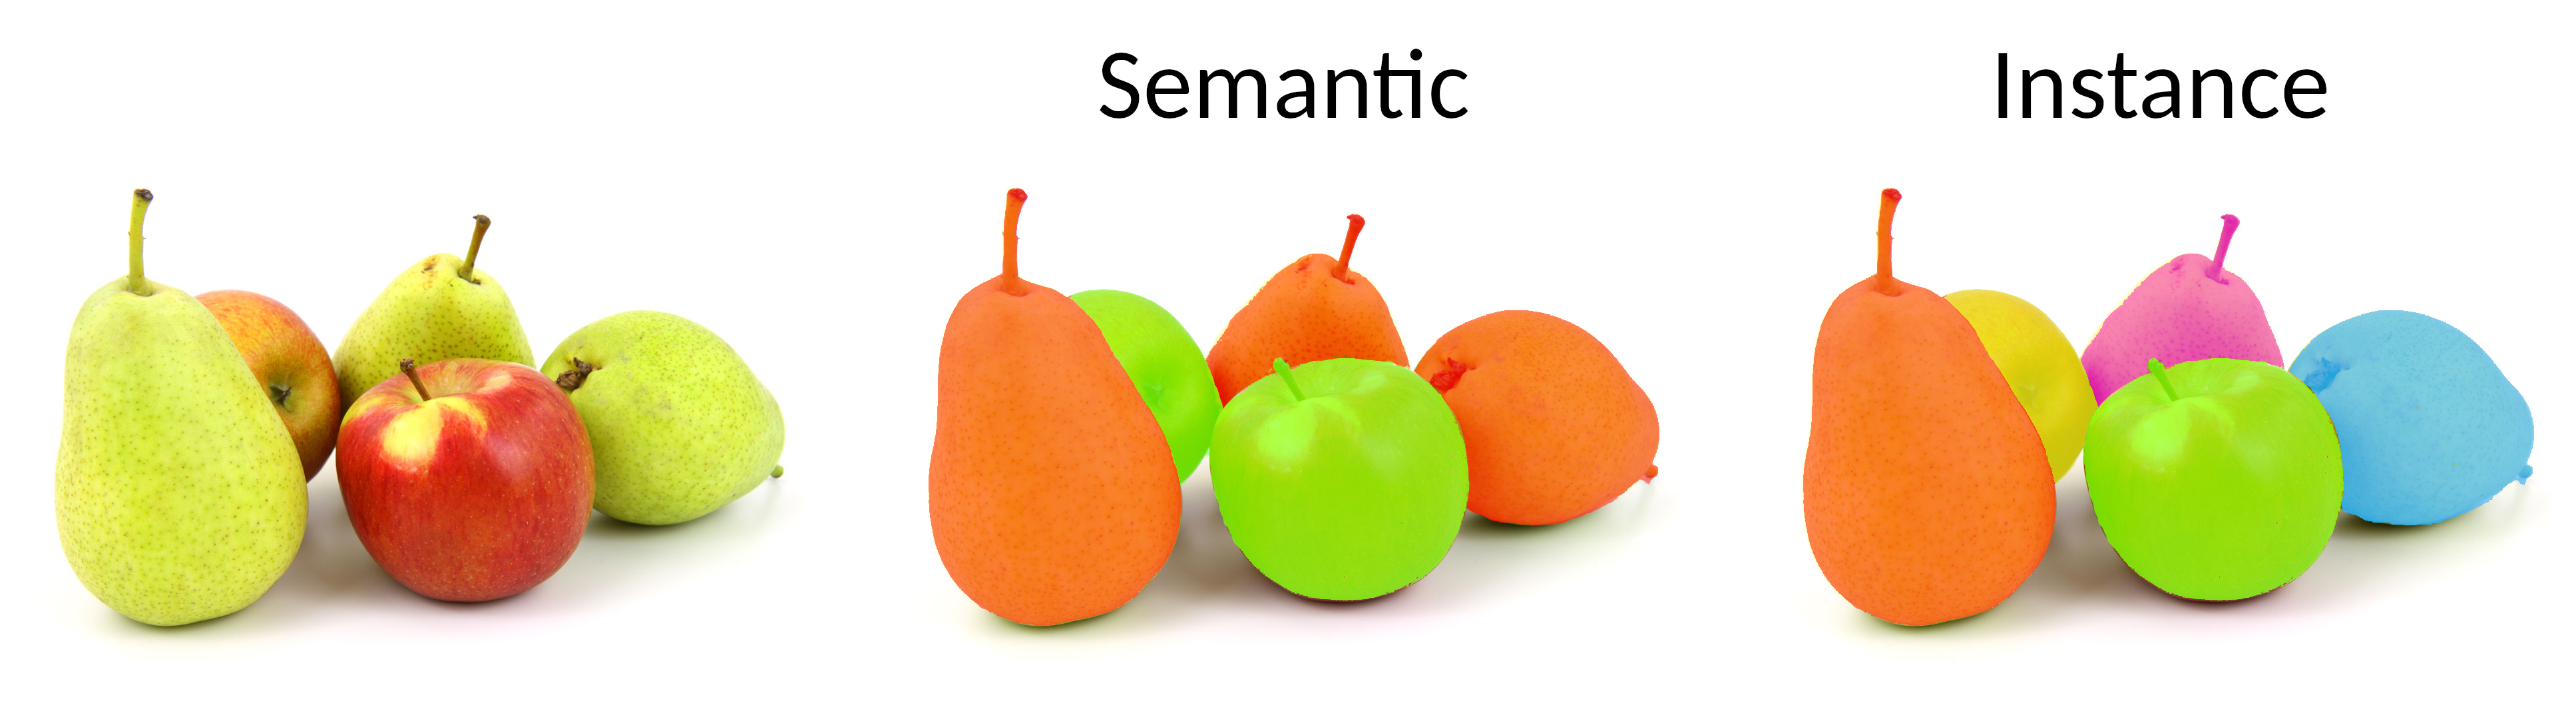
\includegraphics[width=\textwidth]{semantic_vs_instance_cv.jpg}
        \footnotesize
        Source: Apples and pears - Petr Kratochvil - CC0
    }
    \only<2>{
        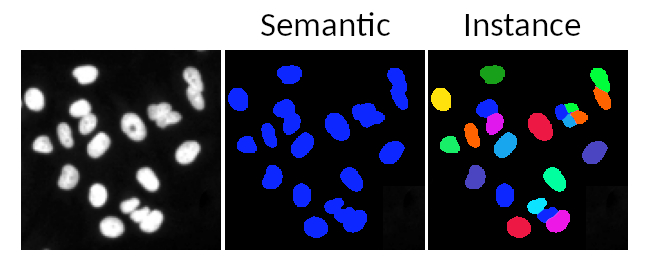
\includegraphics[width=\textwidth]{semantic_vs_instance_bio.jpg}
        \footnotesize
        Source: Nicola Roman\`o
    }
\end{frame}

\section{Semantic segmentation - thresholding methods}

\begin{frame}
    {Thresholding}
    Thresholding is the simplest way of performing semantic segmentation, when there is a clear distinction between the object(s) of interest and the background.

    We define a threshold $t$ and create a mask $M$ such that:

    $$M(x, y) = \begin{cases}
            0 & \text{for}~I(x,y) < t    \\
            1 & \text{for}~I(x,y) \geq t \\
        \end{cases}$$

    \pause
    This can be extended to multi-class segmentation by chosing $t_1, t_2, \dots, t_n$ and generating a mask

    $$M(x, y) = \begin{cases}
            0 & \text{for}~I(x,y) < t_1          \\
            1 & \text{for}~t_1 \leq I(x,y) < t_2 \\
            \dots                                \\
            n & \text{for}~I(x,y) > t_n          \\
        \end{cases}$$
\end{frame}

\begin{frame}
    {Choosing a threshold}
    We can manually choose a threshold by inspecting the image histogram

    \centering
    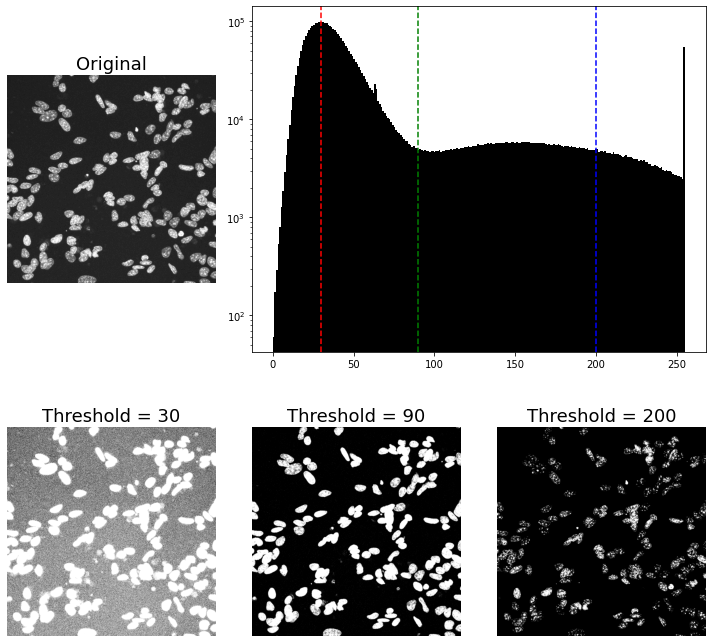
\includegraphics[height=.75\textheight]{manual_thresholding.png}

    \pause
    \textbf{Is there a better way?}
\end{frame}

\begin{frame}
    {Otsu's method}
    Otsu's method is a simple way to automatically choose a threshold.

    The algorithm makes an exhaustive search for the optimal threshold that maximizes the between-class variance (equivalent to minimizing the intra-class variance).

    \large
    $$\sigma_\omega^2 = \omega_0\sigma_0^2+\omega_1\sigma_1^2$$
    $$\omega_0 =\sum_{i=0}^{t-1} p(i)\qquad\omega_1 =\sum_{i=t}^{L-1} p(i)$$
\end{frame}

\begin{frame}
    {Otsu's method - an example}
    \begin{columns}
        \begin{column}{.6\textwidth}
            \begin{codebox}
                \texttt{from skimage.filters import threshold\_otsu\\
                    \\
                    t = threshold\_otsu(img)\\
                    \\
                    plt.imshow(img > t, cmap="gray")\\
                    plt.axis("off")\\
                    plt.title(f"Otsu's threshold (\{t\})", fontsize=18)\\
                    plt.show()}
            \end{codebox}
        \end{column}
        \begin{column}{.4\textwidth}
            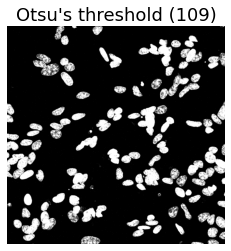
\includegraphics[width=\textwidth]{otsu's threshold.png}
        \end{column}
    \end{columns}
\end{frame}

\begin{frame}
    {Issues with thresholding}

    \begin{itemize}
        \item Noise is a problem -> Gaussian (or median) filter helps
        \item Need to remove holes afterwards
    \end{itemize}
    \centering
    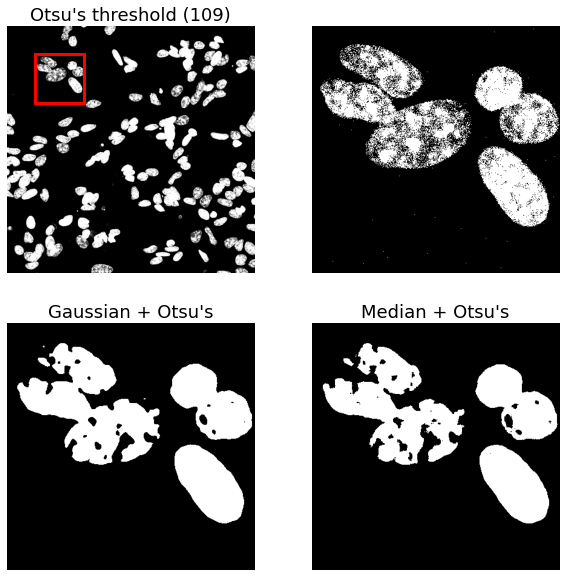
\includegraphics[width=.4\textwidth]{otsu_and_smoothing.png}
\end{frame}

\begin{frame}
    {Filling holes}
    Morphological operations allow to fill small holes.
    The `skimage.morphology.remove\_small\_holes` function is an example of such an operation.

    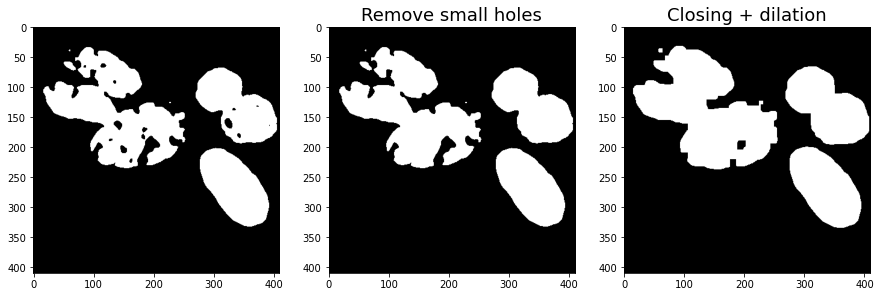
\includegraphics[width=\textwidth]{morphological.png}
\end{frame}
\begin{frame}
    {Multi-Otsu segmentation}
    The Otsu's method can be extended to multi-class segmentation.

    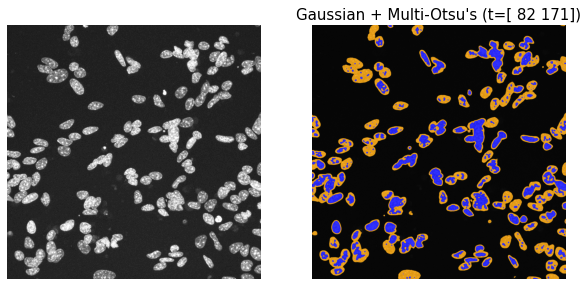
\includegraphics[width=\textwidth]{multiotsu.png}
\end{frame}

\begin{frame}
    {Multi-Otsu segmentation - code}
    \begin{codebox}
        \texttt{from skimage.filters import threshold\_multiotsu, gaussian\\
            from skimage import img\_as\_ubyte\\
            import numpy as np\\
            from skimage.color import label2rgb\\
            \\
            t = threshold\_multiotsu(img, classes=3)\\
            \\
            \pause
            \# Remember to go back to unsigned 8-bit integers from float!\\
            img\_gaus = img\_as\_ubyte(gaussian(img, 5))\\
            \# Convert to mask with 3 levels\\
            img\_thr\_gaus = np.digitize(img\_gaus, t)\\
            \\
            \pause
            \# Handy function to map the labels to colors\\
            img\_with\_overlay = label2rgb(img\_thr\_gaus, image = img, bg\_label=0, colors = ["orange", "blue"], alpha = .8)\\
            \\
            \# Then visualise using Matplotlib!
        }
    \end{codebox}
\end{frame}

\section{Clustering methods}

\begin{frame}
    {k-means segmentation}
    k-means clustering is a popular method for segmentation.

    One of the simplest approaches to clustering
    k-means iteratively divides the dataset in $k$ clusters
\end{frame}

\begin{frame}
    {How k-means works}
    \begin{columns}
        \begin{column}{.5\textwidth}
            \begin{enumerate}[<+->]
                \item We select k random points as the starting centers of the clusters (\textbf{centroids})
                \item We assign each point in the dataset to the closest centroid, according to a distance metric of our choice
                \item We move the centroids to the center of each cluster
                \item We reassign clusters and continue repeating until clusters don’t change anymore or until we reach a certain number of iterations
                \item Most often k-means converges after 10-20 iterations
            \end{enumerate}
        \end{column}
        \begin{column}{.5\textwidth}
            \centering
            \only<1>{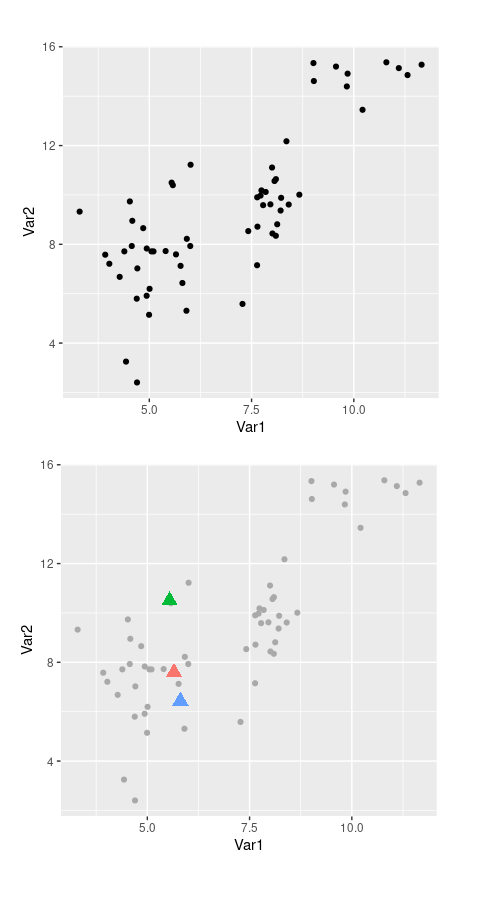
\includegraphics[height=\textheight, trim=0 0 0 -1em]{kmeans-step1.png}}
            \only<2>{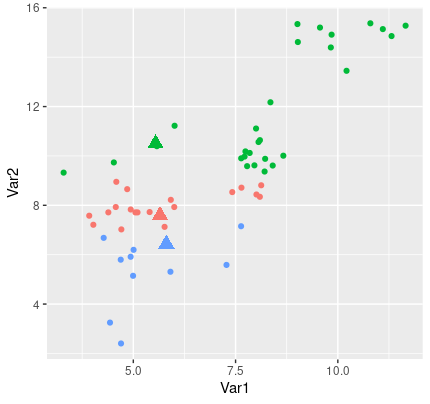
\includegraphics[width=.7\textwidth]{kmeans-step2.png}}
            \only<3>{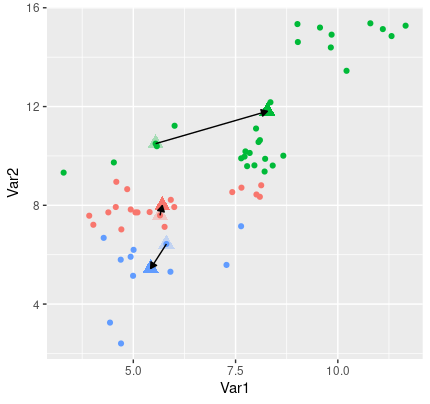
\includegraphics[width=.7\textwidth]{kmeans-step3.png}}
            \only<4->{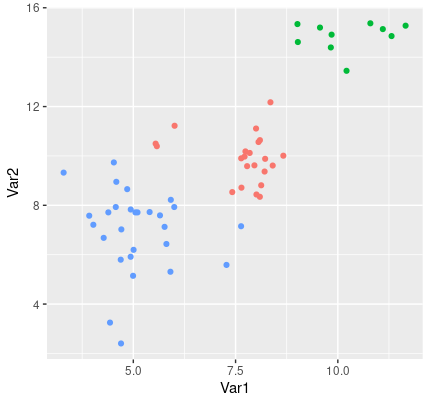
\includegraphics[width=.7\textwidth]{kmeans-final.png}}
        \end{column}
    \end{columns}
\end{frame}

\begin{frame}
    {k-means segmentation - an example}
    \only<1>{
        \centering
        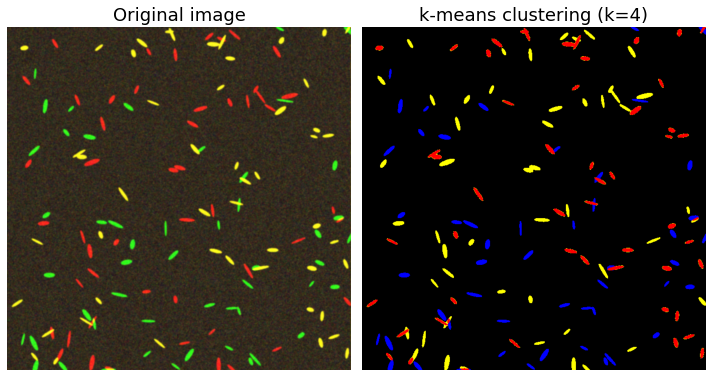
\includegraphics[width=.9\textwidth]{kmeans_on_synthetic_data.png}

        \footnotesize
        Synthetic data simulating cells expressing either or both of a red and green fluorescent protein.
    }
    \only<2>{
        \centering
        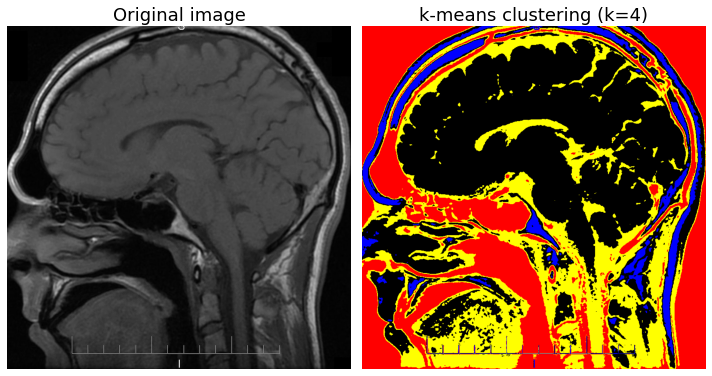
\includegraphics[width=.9\textwidth]{kmeans_MRI.png}

        \footnotesize
        MRI: Bryan Kiechle, CC-BY-NC-2.0
    }
\end{frame}

\begin{frame}
    {k-means segmentation - code}

    \begin{codebox}
        \texttt{from sklearn.cluster import KMeans\\
            from skimage.color import label2rgb\\
            \\
            blobs = imread("blobs\_green\_red.tif")\\
            \\
            \pause
            \# Create k-means model with 4 clusters - set random state for reproducibility\\
            kmeans = KMeans(n\_clusters=4, random\_state=42)\\
            \# Fit the model with our data. We reshape it in 3 columns (R;G;B)\\
            \# For a grayscale image we would reshape to (-1, 1)\\
            kmeans.fit(blobs.reshape(-1, 3))\\
            \# Predict the cluster for each pixel and reshape back to original size.\\
            clusters = kmeans.predict(blobs.reshape(-1, 3))\\
            clusters = clusters.reshape(blobs.shape[0], blobs.shape[1])\\
            \pause
            \\
            plt.imshow(label2rgb(clusters, bg\_label=0))\\
            plt.plot()
        }
    \end{codebox}
\end{frame}

\begin{frame}
    {Fuzzy-C-Means segmentation}
    Fuzzy clustering methods differs from hard clustering (such as k-means) in that data points can belong to multiple clusters, with different probabilities.

    Fuzzy C-Means (FCM) is the most commonly used fuzzy method. It is similar to k-means, but more robust to noise, inconsistent illuminations etc.

    FCM is implemented in the \texttt{FCM} function of the \texttt{fuzzy-c-means} package (imported as \texttt{fcmeans}).
\end{frame}

\begin{frame}
    {FCM example}
    \begin{columns}
        \begin{column}{.5\textwidth}
            \begin{codebox}
                \texttt{fcm = FCM(n\_clusters=n\_clusters, max\_iter=100)\\
                    fcm.fit(img.reshape(-1, 1))\\
                    clusters = fcm.predict(img.reshape(-1, 1))\\
                    clusters = clusters.reshape(img.shape)
                }
            \end{codebox}
        \end{column}
        \begin{column}{.5\textwidth}
            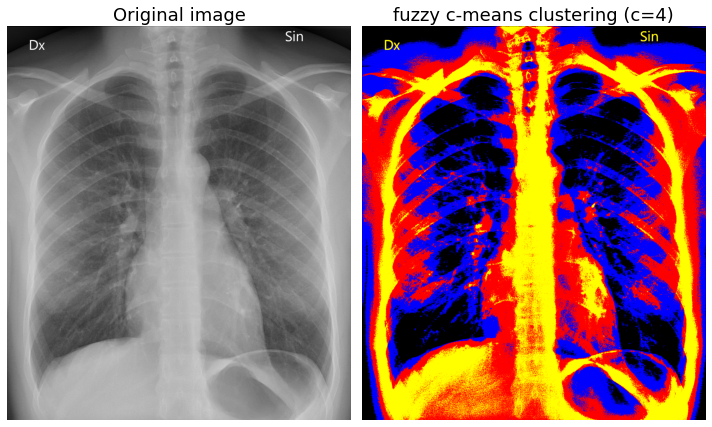
\includegraphics[width=\textwidth]{FCM_xray.png}
        \end{column}
    \end{columns}
\end{frame}
% \begin{frame}
%     {Random walker segmentation}
%     The random walker algorithm segments an image based on markers (either user-defined or automatically calculated).

%     \begin{enumerate}[<+->]
%         \item The algorithm starts with a number of markers for each of the classes we want to segment.
%         \item For each unlabeled pixel we generate a "random walker" and calculate the probability of it reaching one of the markers.
%         \item The random walker is biased to avoid crossing sharp intensity gradient
%         \item We assign each pixel to the class of the marker that it is most likely to reach.
%     \end{enumerate}

%     This is implemented in \texttt{skimage.segmentation.random\_walker} method.
% \end{frame}

% \begin{frame}
%     {Random walker - an example}

% \end{frame}

\section{Instance segmentation}
\begin{frame}
    {Motivation}
    Often we want to measure properties of individual objects in an image.

    In order to do that we need to segment individual instances of the objects.

    We can then create masks for each single object and use it to extract its features (e.g. size, shape, color, intensity etc.).
\end{frame}

\subsection{Watershed}

\begin{frame}
    {Watershed}
    \begin{columns}
        \begin{column}{.6\textwidth}
            The watershed algorithm was developed in 1979 by Beucher and Lantuéjoul.
            \vspace{2em}

            If you consider the image as a surface, the watershed algorithm finds the local minima and starts "flooding the image with water" from these points, until the whole image is covered. It then places "barriers" when water from two minima touches each other.
        \end{column}
        \begin{column}{.4\textwidth}

            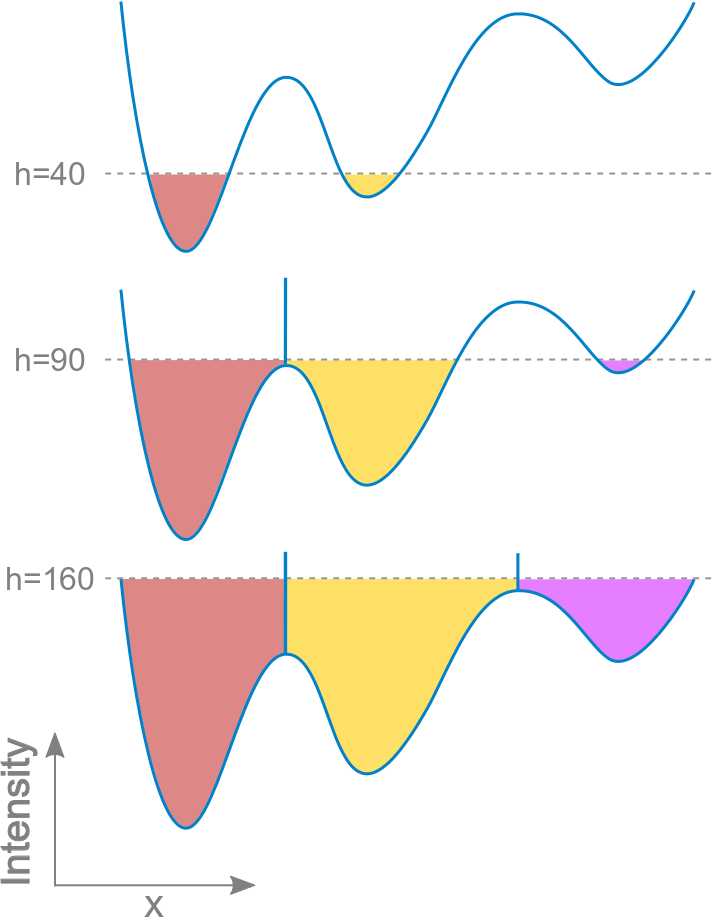
\includegraphics[width=\textwidth, trim = 0 0 0 -5em]{watershed-flooding-graph.png}
            \footnotesize
            Source: ImageJ.net
        \end{column}
    \end{columns}
\end{frame}

\begin{frame}
    {Watershed - an example}
    We are going to segment cell nuclei in an image using the watershed algorithm.

    We will perform the following steps:

    \begin{enumerate}[<+->]
        \item Load the image.
        \item Apply a median filter to remove noise.
        \item Find Otsu's threshold and perform a binary thresholding to isolate nuclei from background.
        \item Apply the Euclidean distance transform to find the pixel-wise distance to the nearest background pixel.
        \item Find local maxima in the distance transform image and mark them as separate regions.
        \item Use the local maxima as starting point for the watershed algorithm.
        \item Perform the watershed algorithm on the distance.
    \end{enumerate}
\end{frame}

\begin{frame}
    {Watershed - code}
    \begin{columns}
        \begin{column}{.7\textwidth}
            \only<-2>
            {
                \begin{codebox}
                    \texttt{\# Import the necessary packages\\
                        from skimage.segmentation import watershed\\
                        from skimage.measure import label\\
                        from skimage.filters import median, threshold\_otsu\\
                        from skimage.morphology import disk\\
                        from skimage.feature import peak\_local\_max\\
                        from skimage.color import label2rgb\\
                        from scipy.ndimage import distance\_transform\_edt\\
                        \\
                        \pause
                        \# Load the image, smooth and threshold\\
                        img = imread("nuclei\_DAPI.tif")\\
                        img\_smooth = median(img, selem=disk(10))\\
                        img\_otsu = img\_smooth > threshold\_otsu(img\_smooth)
                    }
                \end{codebox}
            }
            \only<3->
            {
                \begin{codebox}
                    \texttt{
                        \# Apply the distance transform and find the maxima\\
                        img\_edt = distance\_transform\_edt(img\_otsu)\\
                        peak\_idx = peak\_local\_max(img\_edt, min\_distance=10, exclude\_border=False)\\
                        \# Peaks are returned as coordinates in the original image space,\\
                        \#  so we need to transform them back to the image shape\\
                        peak\_mask = np.zeros\_like(img, dtype=bool)\\
                        peak\_mask[tuple(peak\_idx.T)] = True\\
                        \pause
                        \# Label the peaks and apply the watershed algorithm\\
                        markers = label(peak\_mask)\\
                        img\_watershed = watershed(-img\_edt, markers=markers, mask = img\_otsu)
                    }
                \end{codebox}
            }
        \end{column}
        \begin{column}{.3\textwidth}
            \only<2>{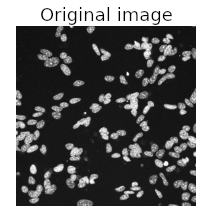
\includegraphics[height=.25\textheight]
                {watershed_process_step1.png}
                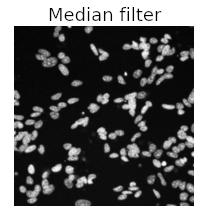
\includegraphics[height=.25\textheight]{watershed_process_step2.png}
                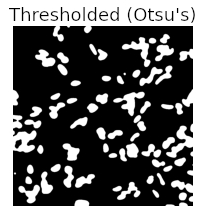
\includegraphics[height=.25\textheight]{watershed_process_step3.png}
            }

            \only<3>{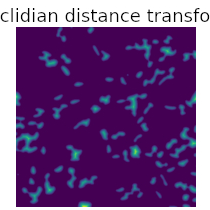
\includegraphics[height=.25\textheight]
                {watershed_process_step4.png}
                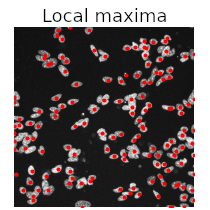
\includegraphics[height=.25\textheight]{watershed_process_step5.png}
                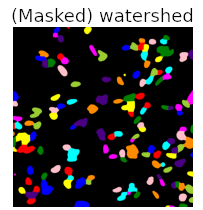
\includegraphics[height=.25\textheight]{watershed_process_step6.png}
            }
        \end{column}
    \end{columns}
\end{frame}

\begin{frame}
    {Measuring region properties}
    Once we have segmented instances, we can measure the properties of each object.
    \vspace{2em}

    \pause

    Scikit image provides the \texttt{regionprops} function in the \texttt{measure} package, that can be used to measure the properties of each region.
    \vspace{2em}

    \pause

    The \texttt{regionprops\_table} function returns the properties in a Pandas-compatible table format. (don't know what Pandas is? Check out Workshop 3!)
\end{frame}

\begin{frame}
    {Measuring properties}
    \begin{codebox}
        \texttt{from skimage.measure import regionprops, regionprops\_table\\
        import pandas as pd\\
        \\
        props = regionprops(img\_watershed, intensity\_image=img)\\
        \\
        areas = [prop.area for prop in props]\\
        intens = [prop.mean\_intensity for prop in props]\\
        \\
        plt.scatter(x=areas, y=intens, color="red")\\
        plt.xlabel("Area")\\
        plt.ylabel("Mean intensity")\\
        plt.plot()\\
        \\
        \pause
        \# Alternatively, with regionprops\_table\\
        tbl = regionprops\_table(img\_watershed, intensity\_image=img, \\
        properties=["area", "mean\_intensity"])      \\
        tbl = pd.DataFrame(tbl)\\
        tbl.to\_csv("cells\_area\_intensity.csv", index=False)
        }
    \end{codebox}
\end{frame}

\begin{frame}
    {What can I measure?}

    A full list of properties can be found in the \href{https://scikit-image.org/docs/dev/api/skimage.measure.html\#skimage.measure.regionprops}{\texttt{\underline{regionprops}}} documentation.

    These include morphological parameters such as area, perimeter, centroid, bounding box/ellipse, mean intensity and many others!
\end{frame}

\end{document}

